\documentclass[convert={outext=.svg,command=\unexpanded{pdf2svg \infile\space\outfile}},multi=false]{standalone}

\usepackage{auto-pst-pdf}
\usepackage{pst-optic}

\usepackage{arev}
\usepackage[T1]{fontenc}
\usepackage{soul}

\begin{document}

%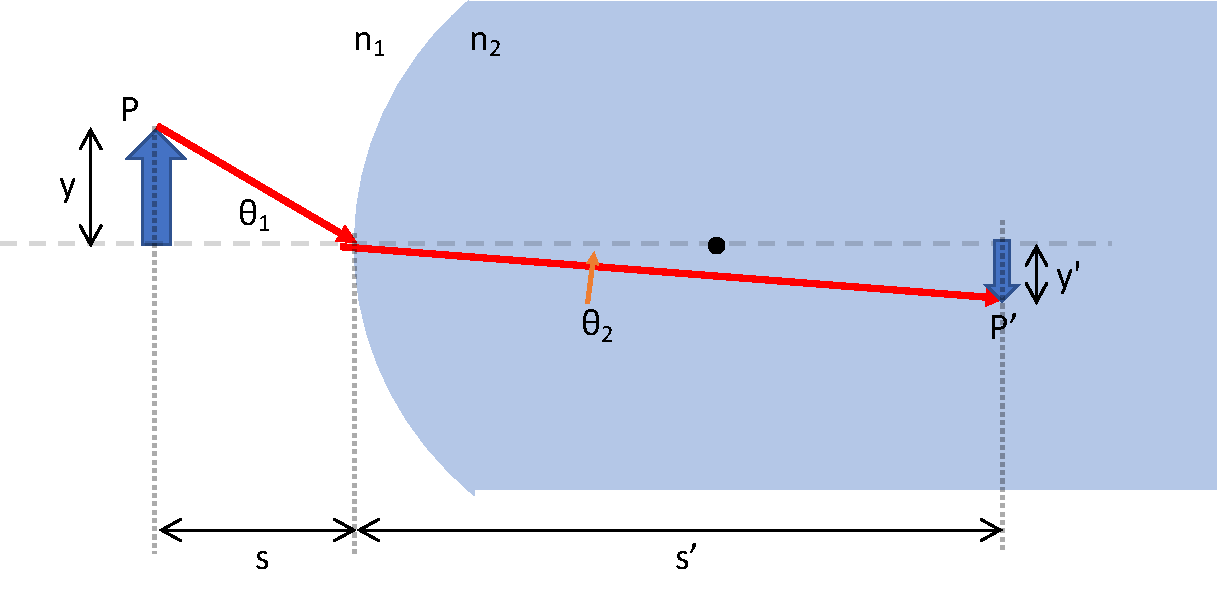
\includegraphics[scale=0.7]{ch16-sphsurfacemag}

\begin{pspicture}[showgrid=false](-10,-2.2)(7,4) 
\rput(0,0){%
\newpsstyle{opticalAxis}{linewidth=0.5pt,linecolor=gray,linestyle=dashed}
\lens[
lensType=DVG,
lensGlass,
lensWidth=0.5,
rayColor=red, 
focus=-3.5,
AB=2,
OA=-7,
spotO=270,
spotAi=270,
spotBi=90,
spotFi=100,
nameFi=F',
]}
\uput[d](-3.5,0){F'}
\uput[d](3.5,0){F}
\psdot*(0,0)
\psdot*(-3.5,0)
\psdot*(3.5,0)

\psline{|<->|,gray}(0,-2)(-7,-2)
\uput[d](-3.5,-2){$s$}
\psline{|<->|,gray}(0,-1.5)(-2.3,-1.5)
\uput[u](-1.15,-1.5){$s'$}

\psline{|<->|,gray}(-7.5,0)(-7.5,2)
\uput[l](-7.5,1){$y$}
\psline{|<->|,gray}(-2,0)(-2,0.669)
\uput[r](-2,0.35){$y'$}

\psline[linecolor=red,linestyle=dashed]{}(0,0.665)(3.5,0)

%\uput[](-1.75,0.25){$\theta$}
%\uput[](1.75,-0.25){$\theta$}
%\ncline{<->}{lens}{object}
%\uput[d](-3,0){F}
\end{pspicture}

\end{document}